\documentclass[a4paper,12pt]{report}

\usepackage{titlesec}
\titleformat{\chapter}[hang]
  {\normalfont\Huge\bfseries} 
  {\thechapter.}             
  {20pt}                     
  {}                         

\usepackage[utf8]{inputenc}
\usepackage[T1]{fontenc}
\usepackage[english, italian]{babel} 

\usepackage{amsmath}

\usepackage{graphicx, xcolor, float}
\graphicspath{{./figures/}} 

\usepackage{listings}
\definecolor{backcolour}{rgb}{0.95,0.95,0.95}
\definecolor{codegreen}{rgb}{0,0.6,0}
\definecolor{codegray}{rgb}{0.5,0.5,0.5}
\definecolor{codepurple}{rgb}{0.58,0,0.82}

\lstset{
    backgroundcolor=\color{backcolour},
    commentstyle=\color{codegreen},
    keywordstyle=\color{blue}\bfseries,
    numberstyle=\tiny\color{codegray},
    stringstyle=\color{codepurple},
    basicstyle=\ttfamily\footnotesize,
    breaklines=true,
    numbers=left,
    showstringspaces=false
}

\renewcommand{\familydefault}{\sfdefault}
\usepackage{eulervm}
\usepackage[colorlinks=true, allcolors=black]{hyperref}

\emergencystretch=1.5em
\pdfsuppresswarningpagegroup=1

\newcommand{\concettoChiave}[1]{\textbf{\textcolor{blue}{#1}}}

\begin{document}

\begin{titlepage}
    \begin{center}
        \vspace*{2cm} 

        \Huge
        \textbf{Corso \LaTeX{} 2026 - Elaborato}

        \vspace{1.5cm}
        
        \Large
        \textbf{Luca Quaresima\\VR500114}

        \vspace*{1cm}
    \end{center}
\end{titlepage}

\tableofcontents

\chapter{Introduzione}

\section{Programmazione Tradizionale}
Fino a poco tempo fa, i programmi informatici seguivano regole rigide e predefinite. Ad esempio, nello sviluppo di un e-commerce, ogni azione dell'utente (come aggiungere un articolo al carrello) corrisponde a una precisa regola codificata a mano dai programmatori. Se un problema può essere risolto interamente con questo approccio deterministico, non c'è alcun bisogno di scomodare l'apprendimento automatico.

\section{I Limiti dell'Approccio Tradizionale}
Molti compiti complessi, tuttavia, non si piegano facilmente all'ingegno umano. Risulta infatti quasi impossibile scrivere da zero, basandosi solo su regole fisse, un programma in grado di:
\begin{itemize} 
    \item Prevedere il meteo analizzando dati satellitari e storici;
    \item Comprendere e rispondere a domande scritte in linguaggio libero;
    \item Identificare e contornare le persone presenti in una fotografia;
    \item Suggerire agli utenti prodotti mirati che non sapevano di desiderare.
\end{itemize}

\section{Cos'è il Machine Learning}
Il \concettoChiave{Machine Learning}
è lo studio di algoritmi capaci di imparare dall'esperienza. A differenza dei software tradizionali che restano statici finché un umano non li aggiorna, questi modelli migliorano le proprie prestazioni man mano che accumulano nuovi dati. Una sua branca fondamentale è il \textit{Deep Learning}, che oggi guida le maggiori innovazioni in campi che vanno dalla computer vision fino alla genomica.

\begin{table}[H]
    \centering
    \begin{tabular}{|l|p{5.5cm}|p{5.5cm}|}
        \hline
        \textbf{Caratteristica} & \textbf{Programmazione Classica} & \textbf{Machine Learning} \\
        \hline
        \textbf{Dati in ingresso} & Dati e regole logiche & Dati ed etichette (esempi) \\
        \textbf{Risultato} & Risposte o decisioni & Modello predittivo \\
        \textbf{Aggiornamento} & Riscrittura del codice sorgente & Riadestramento sui nuovi dati \\
        \textbf{Complessità} & Limitata alla logica umana & Scalabile su problemi complessi \\
        \hline
    \end{tabular}
    \caption{Differenze strutturali tra approccio classico e apprendimento automatico.}
\end{table}


\chapter{Manipolazione dei Dati}

\section{Introduzione ai Tensori}
Per poter ottenere dei risultati, abbiamo bisogno di un modo per memorizzare e manipolare i dati. Iniziamo a sporcarci le mani con gli array $n$-dimensionali, che chiameremo anche \textbf{tensori}. 
Per tutti i moderni framework di deep learning, la classe tensore assomiglia agli \texttt{ndarray} di NumPy, ma con due caratteristiche fondamentali in più:

\begin{itemize}
    \item Supportano la differenziazione automatica.
    \item Sfruttano le GPU per accelerare il calcolo.
\end{itemize}
Tra i framework più popolari troviamo:
\begin{enumerate} 
    \item PyTorch
    \item Tensorflow
    \item JAX
    \item MXNet
\end{enumerate}

\begin{table}[H]
    \centering
    \begin{tabular}{|l|c|c|}
        \hline
        \textbf{Framework} & \textbf{Sviluppatore} & \textbf{Linguaggio Principale} \\
        \hline
        PyTorch & Meta AI & Python / C++ \\
        TensorFlow & Google & Python / C++ \\
        JAX & Google & Python \\
        \hline
    \end{tabular}
    \caption{Confronto tra i principali framework per tensori.}
\end{table}

\section{Primi passi con PyTorch}
Un tensore rappresenta un array (possibilmente multidimensionale) di valori numerici. Nel caso unidimensionale è chiamato \textit{vettore}, con due assi è chiamato \textit{matrice}. Con $k$ assi, ci riferiamo all'oggetto semplicemente come un tensore di ordine $k$.\\
Iniziamo importando la libreria. Tramite la funzione \texttt{arange(n)}, possiamo creare un vettore di valori equidistanti:

\begin{lstlisting}[language=Python]
import torch
x = torch.arange(12, dtype=torch.float32)
print(x)    
\end{lstlisting}

Possiamo cambiare la forma (shape) di un tensore senza alterarne la dimensione o i valori usando \texttt{reshape}. Da un punto di vista matematico, se consideriamo un tensore multidimensionale di dimensioni $d_1 \times d_2 \times \dots \times d_k$, il numero totale di elementi $N$ è dato dal prodotto delle singole dimensioni. Quando esequiamo un'operazione di rimodellamento (reshape) in una nuova forma a $m$ dimensioni $(R_1, R_2, \dots, R_m)$, la cardinalità complessiva deve rimanere invariata:

\begin{equation}
    N = \prod_{i=1}^{k} d_i = \prod_{j=1}^{m} R_j
\end{equation}

Nel caso specifico di una trasformazione da vettore a matrice bidimensionale di forma $(R, C)$, l'equazione si semplifica e ci permette di ricavare il vincolo strutturale:
\begin{equation}
    N = R \times C \implies C = \frac{N}{R}
\end{equation}

Ecco come appare l'applicazione pratica di questo concetto tramite codice:

\begin{lstlisting}[language=Python]
X = x.reshape(3, 4)
print(X)
\end{lstlisting}

\begin{figure}[H]
    \centering
    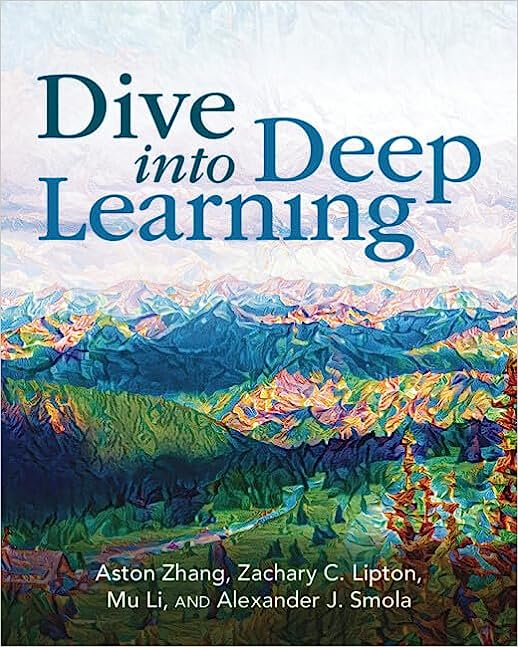
\includegraphics[width=0.5\textwidth]{d2l.jpg} 
    \caption{Testo di riferimento.}
\end{figure}

\end{document}